\documentclass[12pt,a4paper]{report}

% ==========================================
% LATEX PACKAGES
% ==========================================
\usepackage[utf8]{inputenc}
\usepackage[margin=1in]{geometry}
\usepackage{graphicx}
\usepackage{hyperref}
\usepackage{titlesec}
\usepackage{setspace}
\usepackage{longtable}
\usepackage{float}
\usepackage{booktabs}
\usepackage{array}
\usepackage{listings}
\usepackage{xcolor}
\usepackage{fancyhdr}
\usepackage{amsmath}
\usepackage{newtxtext}
\usepackage{newtxmath}
\usepackage{enumitem}
\usepackage{cite}

% ==========================================
% DOCUMENT FORMATTING & STYLING (Strict guidelines)
% ==========================================
\setstretch{1.2}
\hypersetup{
    colorlinks=true,
    linkcolor=blue,
    filecolor=magenta,      
    urlcolor=cyan,
    pdftitle={AI-Powered Personal Financial Advisor},
    pdfpagemode=FullScreen,
}

% Bullet formatting rules: Use only (a), (b), (c) or (i), (ii), (iii)
\setlist[enumerate,1]{label=(\alph*)}
\setlist[enumerate,2]{label=(\roman*)}

% Compact spacing
\setlength{\textfloatsep}{8pt}
\setlength{\floatsep}{6pt}
\setlength{\intextsep}{6pt}
\setlength{\abovecaptionskip}{3pt}
\setlength{\belowcaptionskip}{2pt}
\setlength{\parskip}{2pt plus 1pt minus 1pt}
\setlength{\parindent}{18pt}

% Header heights
\pagestyle{fancy}
\setlength{\headheight}{15pt}
\fancyhf{}
\fancyhead[L]{\slshape \leftmark}
\fancyhead[R]{\thepage}
\renewcommand{\headrulewidth}{0.4pt}

% Headings styling (Strict guidelines: Size 16 bold uppercase for main, 14 bold for section)
\titleformat{\chapter}[block]
  {\normalfont\fontsize{16}{20}\bfseries\filcenter}
  {CHAPTER \thechapter\\}
  {0.5em}
  {\uppercase}
\titlespacing*{\chapter}{0pt}{-20pt}{20pt}

\titleformat{\section}
  {\normalfont\fontsize{14}{18}\bfseries}
  {\thesection}
  {1em}
  {}
\titlespacing*{\section}{0pt}{12pt}{6pt}

\titleformat{\subsection}
  {\normalfont\fontsize{12}{15}\bfseries}
  {\thesubsection}
  {1em}
  {}
\titlespacing*{\subsection}{0pt}{8pt}{4pt}

% Code listing styles
\definecolor{codegreen}{rgb}{0,0.6,0}
\definecolor{codegray}{rgb}{0.5,0.5,0.5}
\definecolor{codepurple}{rgb}{0.58,0,0.82}
\definecolor{backcolour}{rgb}{0.96,0.96,0.94}

\lstdefinestyle{mystyle}{
    backgroundcolor=\color{backcolour},   
    commentstyle=\color{codegreen},
    keywordstyle=\color{blue},
    numberstyle=\tiny\color{codegray},
    stringstyle=\color{codepurple},
    basicstyle=\ttfamily\footnotesize,
    breakatwhitespace=false,         
    breaklines=true,                 
    captionpos=b,                    
    keepspaces=true,                 
    numbers=left,                    
    numbersep=5pt,                  
    showspaces=false,                
    showstringspaces=false,
    showtabs=false,                  
    tabsize=2
}
\lstset{style=mystyle, aboveskip=6pt, belowskip=6pt}

\lstdefinelanguage{JavaScript}{
  keywords={break, case, catch, continue, debugger, default, delete, do, else, false, finally, for, function, if, in, instanceof, new, null, return, switch, this, throw, true, try, typeof, var, void, while, with, let, const, async, await},
  morecomment=[l]{//},
  morecomment=[s]{/*}{*/},
  morestring=[b]',
  morestring=[b]"
}
\lstdefinelanguage{json}{
  literate=
    *{:}{{{\color{blue}{:}}}}{1}
     {,}{{{\color{blue}{,}}}}{1}
     {\{}{{{\color{blue}{\{}}}}{1}
     {\}}{{{\color{blue}{\}}}}}{1}
     {[}{{{\color{blue}{[}}}}{1}
     {]}{{{\color{blue}{[}}}}{1},
  morestring=[b]"
}

% ==========================================
% DOCUMENT CONTENT
% ==========================================
\begin{document}

% --- COVER PAGE ---
\begin{titlepage}
\begin{center}
    \singlespacing
    \large
    \textbf{Applied AI PROJECT REPORT}\\
    \textbf{on}\\
    \vspace{0.8cm}
    \Large
    \textbf{AI-Powered Personal Financial Advisor using n8n, Ollama and Multi-Agent Architecture}\\
    \vspace{1.5cm}
    \large
    \textit{Submitted as partial fulfillment of}\\
    \vspace{0.5cm}
    \textbf{MASTER OF COMPUTER APPLICATION DEGREE}\\
    \vspace{0.8cm}
    \textbf{SESSION 2025-26}\\
    \vspace{1.2cm}
    \textit{By}\\
    \vspace{0.3cm}
    \textbf{Apeksha Goel}\\
    \textbf{(2503201450028)}\\
    \vspace{1.5cm}
    \textit{Under the guidance of}\\
    \vspace{0.5cm}
    \noindent
    \begin{minipage}[t]{0.45\textwidth}
        \centering
        \textbf{Priya Mishra}\\
        Asst. Prof. (Sr. Scale)
    \end{minipage}
    \hfill
    \begin{minipage}[t]{0.45\textwidth}
        \centering
        \textbf{Alpana Lodhi}\\
        Asst. Prof.
    \end{minipage}
    \vspace{1.5cm}

    \begin{figure}[H]
        \centering
        
\includegraphics[width=3.5cm]{images/abes_logo.png}
    \end{figure}
    \vspace{0.5cm}
    \textbf{ABES ENGINEERING COLLEGE, GHAZIABAD (032)}\\
    \vspace{0.3cm}
    \textit{AFFILIATED TO}\\
    \vspace{0.3cm}
    \textbf{Dr. A.P.J. ABDUL KALAM TECHNICAL UNIVERSITY, UTTAR PRADESH, LUCKNOW}
\end{center}
\end{titlepage}

% --- PRELIMINARY PAGES ---
\pagenumbering{roman}
\setcounter{page}{1}

% Certificate
\newpage
\begin{center}
    \Large\textbf{CERTIFICATE}\\
    \vspace{1.0cm}
\end{center}
\onehalfspacing
This is to certify that the Applied AI Project Report entitled \textbf{``AI-Powered Personal Financial Advisor using n8n, Ollama and Multi-Agent Architecture''} is a record of work carried out by \textbf{Apeksha Goel} (Roll Number: \textbf{2503201450028}) under our supervision in partial fulfillment of the requirements for the award of the degree of Master of Computer Application (MCA) from ABES Engineering College, Ghaziabad, affiliated to Dr. A.P.J. Abdul Kalam Technical University, Lucknow.
\vspace{1.5cm}

\noindent
\begin{minipage}[t]{0.45\textwidth}
    \centering
    \textbf{Priya Mishra}\\
    Asst. Prof. (Sr. Scale)\\
    Internal Guide
\end{minipage}
\hfill
\begin{minipage}[t]{0.45\textwidth}
    \centering
    \textbf{Alpana Lodhi}\\
    Asst. Prof.\\
    Co-Guide
\end{minipage}

\vspace{1.5cm}
\noindent
\begin{minipage}[t]{1.0\textwidth}
    \centering
    \textbf{Head of Department}\\
    Department of MCA\\
    ABES Engineering College, Ghaziabad
\end{minipage}


% --- CHAPTERS ---
\clearpage
\pagenumbering{arabic}
\setcounter{page}{1}

\chapter{Introduction}
In the modern economic landscape, financial planning has shifted from manual bookkeeping to digital advisory systems. Individuals face significant personal finance challenges, such as tracking diverse investments, establishing emergency reserves, evaluating loan amortization schedules, and selecting optimal tax regime paths. The complexity of financial planning often leads to cognitive fatigue, causing delayed decisions or financial mismanagement. Navigating these challenges requires specialized knowledge that is typically gatekept by high advisory fees or inaccessible financial planners.

AI-powered advisory systems have emerged as a powerful solution. Large Language Models (LLMs) act as reasoning engines capable of parsing unstructured inputs, understanding intent, and generating customized advice in natural language. Running LLMs on cloud servers is common, but raises serious concerns regarding financial data privacy and monthly subscription costs. For an individual, sharing granular detail of monthly income, outstanding debts, and personal savings targets with commercial cloud APIs poses security hazards.

To overcome this, local LLM execution via Ollama allows users to run models (such as Llama 3.2 3B) locally on consumer hardware, keeping personal financial information completely secure within the user's local network. Additionally, node-based automation platforms like n8n provide a visual orchestrator to connect triggers, memories, tools, and agents into sequential, collaborative pipelines without complex coding interfaces. This project presents a unified local framework that combines the visual orchestration of n8n with local Ollama models to build a privacy-first personal financial advisor.

\section{Objective}
The primary objective of this project is to develop a complete visual and local multi-agent chatbot system that automates the collection and synthesis of personal financial analyses:
\begin{enumerate}
    \item \textbf{Budget Analysis}: Automate the extraction of monthly income and expenses from natural queries to compute cash flows, formulate 50-30-20 budget allocations (Needs, Wants, and Savings), and establish target emergency fund sizes equivalent to 6 months of basic expenses.
    \item \textbf{Investment Recommendations}: Implement systematic investment plan (SIP) simulation tools to compute compounding wealth results, analyzing long-term mutual funds, equity allocations, gold holdings, and Public Provident Fund (PPF) deposits.
    \item \textbf{Loan Analysis}: Calculate monthly Equated Monthly Installment (EMI) values, loan repayment schedules, and interest rates, suggesting optimal payoff strategies such as the debt snowball (paying lowest balance first) or debt avalanche (paying highest interest rate first).
    \item \textbf{Tax Optimization}: Model tax calculations under the Old and New tax regimes (specifically focusing on Indian tax structures), guiding users on legal deductions under Sections 80C and 80D.
    \item \textbf{Automated Report Generation}: Combine findings from specialized agents into a single report, formatted as a JSON object mapping recommendations, risks, and action items, returned directly to the user interface.
\end{enumerate}

\section{Need of Project}
The development of this project is driven by several key factors in the personal finance sector:
\begin{enumerate}
    \item \textbf{Lack of Affordable Financial Advisors}: Professional wealth management services are expensive and often targeted exclusively at high-net-worth individuals, leaving middle-class and low-income earners without guidance.
    \item \textbf{Personalized Finance Planning}: Static calculators on websites are rigid, requiring structured inputs. This project uses AI to interpret natural, unstructured expressions and build personalized plans dynamically based on the user's specific context.
    \item \textbf{Automation Benefits}: Linking budget margins directly to investment targets prevents unrealistic financial plans (e.g. recommending a high SIP that exceeds the user's monthly surplus). It automates what would otherwise require multiple independent spreadsheet formulas.
    \item \textbf{AI-driven Decision Support}: LLMs act as cognitive interfaces that guide users through budgeting, tax, and debt scenarios, providing a user-friendly way to navigate complex financial rules and math calculations.
    \item \textbf{Data Privacy and Trust}: Traditional financial portals sell user data to credit bureaus and lenders. A fully local system running via Ollama creates a trust barrier, ensuring the user's private data remains completely private.
\end{enumerate}

\chapter{Requirements}
This chapter specifies the hardware configurations and software runtime environments required to execute the multi-agent chatbot system and host local LLM inference. Selecting appropriate requirements is crucial for guaranteeing low-latency response generation and avoiding memory crashes during execution.

\section{Hardware Requirements}
Running Large Language Models (LLMs) locally requires sufficient hardware resources, particularly processor cores and system memory (RAM). The weights of the Llama 3.2 3B parameter model are loaded directly into RAM (or VRAM if a dedicated GPU is available). Insufficient memory leads to system page faults or crashes during inference. The hardware specifications are listed in Table \ref{table:hardware_req}.

\begin{table}[H]
    \centering
    \caption{Hardware Configuration Specifications}
    \label{table:hardware_req}
    \begin{tabular}{lll}
        \toprule
        \textbf{Component} & \textbf{Minimum Specification} & \textbf{Recommended Specification} \\
        \midrule
        Processor & Intel Core i5 / AMD Ryzen 5 (4 Cores) & Intel Core i7 / AMD Ryzen 7 (8 Cores) \\
        System RAM & 8 GB DDR4 & 16 GB DDR4 / DDR5 \\
        Storage Space & 20 GB Free SSD Storage & 40 GB Free NVMe SSD Storage \\
        Network & 1 Mbps (for setup) & 10 Mbps+ High-speed Broadband \\
        Graphics (Optional) & Shared Integrated Graphics & Dedicated GPU with 6GB+ VRAM \\
        \bottomrule
    \end{tabular}
\end{table}

The memory footprint of running Ollama with Llama 3.2 3B is approximately 2.2 GB. Under Windows, the operating system utilizes 3-4 GB of RAM, leaving the remaining capacity for the runtime processes of n8n, Python, and the web browser interface. High-speed SSD storage is recommended to decrease model loading times from disk into RAM when the Ollama service starts.

\section{Software Requirements}
The multi-agent orchestration pipeline is built using node-based automation platforms, Python scripting libraries, and local model servers. The software components are listed in Table \ref{table:software_req}.

\begin{table}[H]
    \centering
    \caption{Software Environment Specifications}
    \label{table:software_req}
    \begin{tabular}{llp{7.5cm}}
        \toprule
        \textbf{Software} & \textbf{Version} & \textbf{Purpose} \\
        \midrule
        Windows 11 & 64-bit & Operating system platform for the local deployment. \\
        Python & 3.11+ & Programming runtime for testing utilities and CrewAI script. \\
        Ollama & v0.1.48+ & Hosting and serving local LLM models (e.g. Llama 3.2 3B). \\
        n8n & v2.8.4 & Node-based visual multi-agent workflow manager. \\
        CrewAI & v0.28+ & Python multi-agent orchestration framework. \\
        LangChain & v0.1.0+ & Library for connecting local tools and model bindings. \\
        VS Code & v1.85+ & Integrated Development Environment (IDE) for custom code. \\
        Streamlit & v1.30+ & Web framework used to build the advisor user interface. \\
        \bottomrule
    \end{tabular}
\end{table}

\begin{enumerate}
    \item \textbf{n8n Visual Workflow Engine}: Functions as the central API gateway and orchestrator. It executes the sequential agent chain, handles webhook triggers, maintains memory state, and executes Javascript tools.
    \item \textbf{Ollama Local Model Server}: Exposes a local API endpoint on port 11434, executing model inference requests.
    \item \textbf{CrewAI and LangChain Frameworks}: Used during the prototype design phase to validate agent role-play configurations and sequential task execution in Python before porting the logic to n8n nodes.
    \item \textbf{Streamlit User Interface}: Provides a clean web form for users to interact with the chatbot, sending webhook queries and rendering the structured advisory output.
\end{enumerate}

\chapter{Methodology}
The implementation methodology consists of three distinct phases: setting up a local LLM agent with Ollama, configuring a multi-agent collaboration workflow using CrewAI, and designing a production-grade sequential agent pipeline in n8n. The integration of mathematical calculator tools with language models is key to resolving mathematical inaccuracies (hallucinations) common in deep learning models.

\section{Write Agent using Ollama}
The foundation of our system is the deployment of local Large Language Models (LLMs) on consumer-grade hardware. Ollama serves as a local inference runner, hosting the Llama 3.2 3B parameter model and exposing a standardized API endpoint on port 11434. 

To build an agent, we write Python wrappers that interface with this endpoint, handling variable formatting and system prompts. Prompt engineering is used to control output style and temperature. Listing \ref{lst:ollama_agent} shows a Python wrapper for generating structured single-agent queries.

\begin{lstlisting}[language=Python, caption=Python Implementation of Local Ollama Agent, label=lst:ollama_agent]
import urllib.request
import json

class LocalOllamaAgent:
    def __init__(self, model_name="llama3.2", base_url="http://localhost:11434"):
        self.model_name = model_name
        self.base_url = f"{base_url}/api/generate"

    def invoke(self, system_prompt, user_query):
        payload = {
            "model": self.model_name,
            "prompt": f"System: {system_prompt}\nUser: {user_query}\nResponse:",
            "stream": False,
            "options": {
                "temperature": 0.2
            }
        }
        
        req = urllib.request.Request(
            self.base_url,
            data=json.dumps(payload).encode("utf-8"),
            headers={"Content-Type": "application/json"}
        )
        
        try:
            with urllib.request.urlopen(req) as response:
                res_data = json.loads(response.read().decode("utf-8"))
                return res_data.get("response", "")
        except Exception as e:
            return f"Error connecting to Ollama: {str(e)}"

# Example usage
if __name__ == "__main__":
    agent = LocalOllamaAgent()
    sys_msg = "You are a budgeting expert. Format your reply in one line."
    reply = agent.invoke(sys_msg, "I earn 50000 and spend 30000. What is my savings rate?")
    print("Agent Response:", reply)
\end{lstlisting}

\section{Multi-agents with LangChain, CrewAI and Ollama}
While a single model handles basic text generation, multi-agent frameworks are required to model complex scenarios that require distinct personas, guidelines, and access to tools. The CrewAI framework is used to define role-playing agents, configure task assignments, and orchestrate collaboration. LangChain binds our local Ollama model to the CrewAI framework.

The agents execute tasks sequentially:
\begin{enumerate}
    \item \textbf{Budget Agent}: Analyzes the user query and runs the budgeting tool to calculate surpluses.
    \item \textbf{Investment Agent}: Formulates asset allocations using compounding projections.
    \item \textbf{Debt Agent}: Resolves EMI payment terms and payoff methods.
    \item \textbf{Tax Agent}: Evaluates regime efficiency (Old vs New).
\end{enumerate}

Listing \ref{lst:crewai_multiagent} details the implementation of a collaborative multi-agent financial advisor system in CrewAI.

\begin{lstlisting}[language=Python, caption=Multi-Agent Collaboration in CrewAI, label=lst:crewai_multiagent]
from crewai import Agent, Task, Crew, Process, LLM
from langchain.tools import tool

# Define local Ollama configuration via LangChain-compatible CrewAI LLM wrapper
local_llm = LLM(
    model="ollama/llama3.2:3b",
    base_url="http://localhost:11434"
)

@tool("budget_calculator")
def budget_calculator(monthly_income: float, monthly_expenses: float) -> str:
    """Calculates savings surplus and emergency fund target."""
    surplus = monthly_income - monthly_expenses
    emergency_fund = monthly_expenses * 6
    return f"Surplus: {surplus}, Emergency Target: {emergency_fund}"

# Define Agents
budget_agent = Agent(
    role="Budgeting Specialist",
    goal="Analyze cash flows and establish budget targets.",
    backstory="You evaluate spending behaviors and emergency preparedness.",
    tools=[budget_calculator],
    llm=local_llm,
    verbose=True
)

investment_agent = Agent(
    role="Investment Strategist",
    goal="Identify wealth-creation opportunities and run compounding plans.",
    backstory="Senior advisor focused on mutual funds, gold, and PPF allocations.",
    llm=local_llm,
    verbose=True
)

# Define Tasks
budget_task = Task(
    description="Analyze query: 'I earn 50000 and spend 30000.' Run the calculator.",
    expected_output="A structured report mapping surplus and emergency fund sizes.",
    agent=budget_agent
)

investment_task = Task(
    description="Develop compounding recommendations based on the budget analysis.",
    expected_output="An allocation plan showing long-term investment goals.",
    agent=investment_agent
)

# Assemble Crew
financial_crew = Crew(
    agents=[budget_agent, investment_agent],
    tasks=[budget_task, investment_task],
    process=Process.sequential
)

result = financial_crew.kickoff()
print("Crew Final Output:", result)
\end{lstlisting}

\section{Multi-agent using n8n and Ollama}
To build a production system, we deploy the multi-agent architecture in n8n. This platform provides visual debugging, webhook routing, database integrations, and JSON parsing tools. Figure \ref{fig:n8n_workflow} displays the visual multi-agent personal financial advisor workflow implemented in n8n.

\begin{figure}[H]
    \centering
    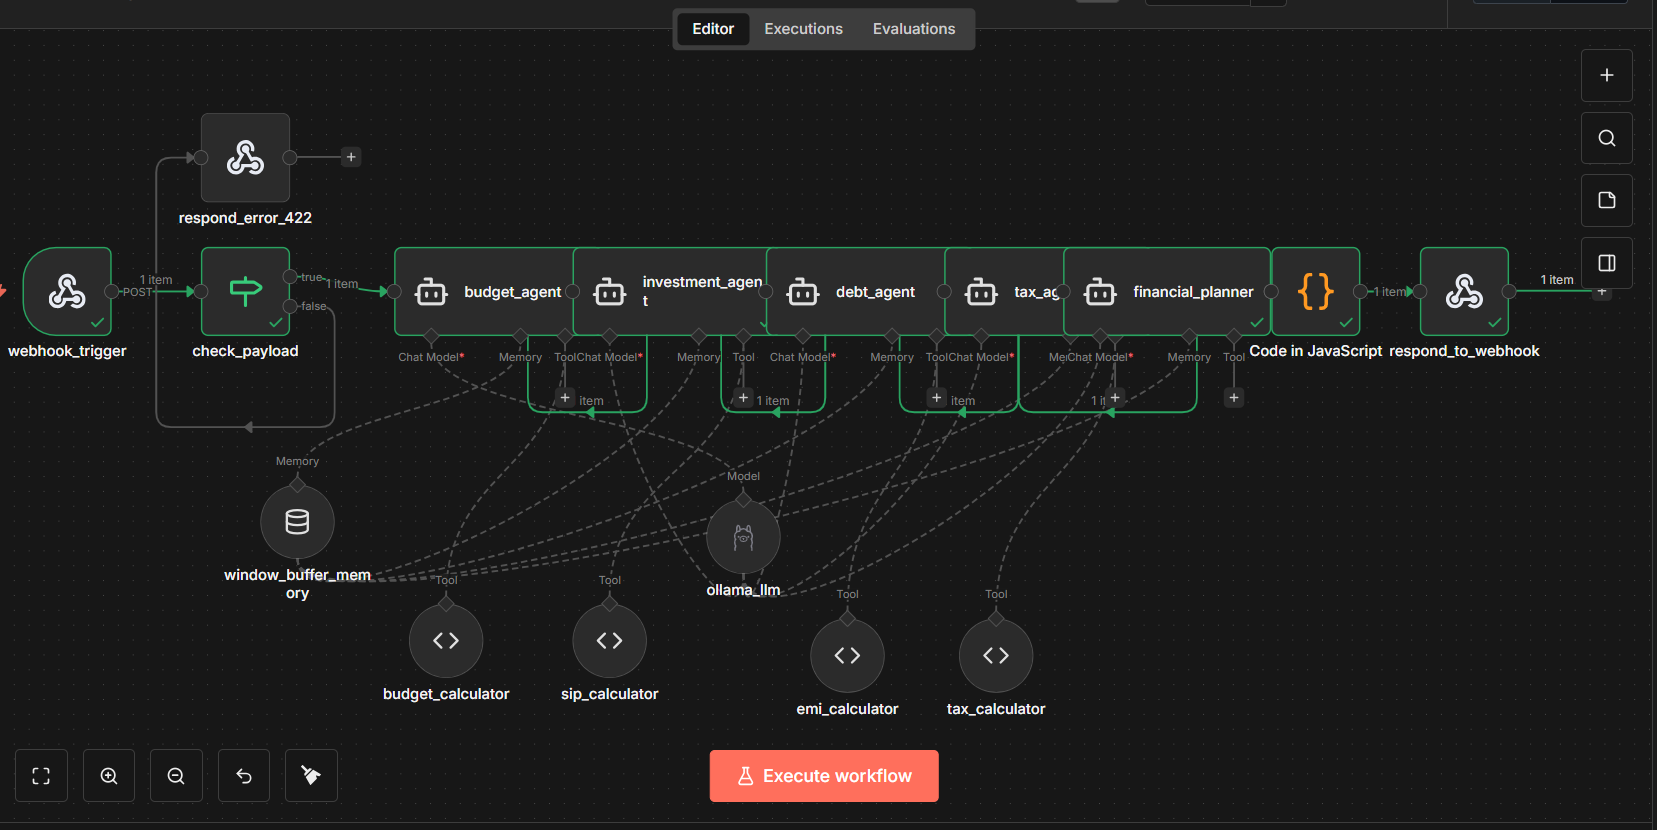
\includegraphics[width=0.95\textwidth]{images/n8n_Personal_Financial_Agent.png}
    \caption{Multi-Agent Workflow Implemented in n8n}
    \label{fig:n8n_workflow}
\end{figure}

The node execution flow operates as follows:
\begin{enumerate}
    \item \textbf{Trigger Node}: An HTTP POST Webhook node accepting parameters (\texttt{session\_id} and \texttt{message}) on the \texttt{/webhook/finance-advisor} endpoint.
    \item \textbf{Check Payload (IF Node)}: A validation node that verifies the presence of parameters.
    \item \textbf{Financial Analysis Agent (Budget Agent)}: Evaluates the query using the custom JS \texttt{budget\_calculator} tool.
    \item \textbf{Investment Agent}: Builds mutual fund and PPF recommendations using the JS \texttt{sip\_calculator} tool.
    \item \textbf{Loan Agent (Debt Agent)}: Formulates payment schedules using the JS \texttt{emi\_calculator} tool.
    \item \textbf{Tax Agent}: Calculates tax efficiency comparison using the JS \texttt{tax\_calculator} tool.
    \item \textbf{Report Generator Agent (Financial Planner)}: Combines all outputs into a single JSON object.
\end{enumerate}

To prevent validation crashes common to lightweight local models (which occasionally format numbers as strings), the custom JS tools are mapped to a relaxed schema: \texttt{["number", "string", "null"]}. Table \ref{table:tool_schemas} details the inputs accepted by these calculators.

\begin{table}[H]
    \centering
    \caption{Custom Tool Schemas}
    \label{table:tool_schemas}
    \begin{tabular}{lllp{6cm}}
        \toprule
        \textbf{Tool Name} & \textbf{Parameter} & \textbf{Type} & \textbf{Description} \\
        \midrule
        budget\_calculator & monthly\_income & [number, string, null] & Monthly earnings. \\
        & monthly\_expenses & [number, string, null] & Monthly expenditure. \\
        \midrule
        sip\_calculator & monthly\_investment & [number, string, null] & Monthly SIP contribution. \\
        & expected\_return\_rate & [number, string, null] & Annual yield rate. \\
        & years & [number, string, null] & Investment timeline in years. \\
        \midrule
        emi\_calculator & principal & [number, string, null] & Total loan principal. \\
        & annual\_interest\_rate & [number, string, null] & Annual loan rate percentage. \\
        & years & [number, string, null] & Repayment tenure in years. \\
        \midrule
        tax\_calculator & annual\_income & [number, string, null] & Total yearly taxable earnings. \\
        \bottomrule
    \end{tabular}
\end{table}

Each of the custom tools is implemented with deterministic mathematical algorithms to ground the language model's reasoning:
\begin{enumerate}
    \item \textbf{Budget Calculator}: Evaluates monthly surplus and savings rate. It projects the popular 50-30-20 budget allocation scheme (allocating 50\% of monthly income to core Needs, 30\% to optional Wants, and 20\% to Savings) and calculates a 6-month emergency reserve cushion based on monthly expenses.
    \item \textbf{SIP Calculator}: Simulates systematic monthly investment plans by executing the Future Value of an Annuity Due formula:
    \[
    FV = P \times \left( \frac{(1 + r)^n - 1}{r} \right) \times (1 + r)
    \]
    where $P$ is the monthly investment, $r$ is the monthly expected return rate, and $n$ is the total number of months. It outputs the total invested capital, final maturity value, and compound wealth gained over the tenure.
    \item \textbf{EMI Calculator}: Resolves loan amortization parameters. It executes the standard amortization formula to calculate the monthly payment:
    \[
    EMI = P \times \frac{r(1+r)^n}{(1+r)^n - 1}
    \]
    where $P$ is the loan principal, $r$ is the monthly interest rate, and $n$ is the total number of months. It calculates the total interest payable and repayment totals.
    \item \textbf{Tax Calculator}: Models yearly income tax obligations under the Indian Tax Slab rules. Under the New Regime (FY 2024-25), it deducts a standard deduction of INR 75,000 and calculates tax progressively (5\% for 3L--6L, 10\% for 6L--9L, 15\% for 9L--12L, 20\% for 12L--15L, and 30\% above 15L). Under the Old Regime, it applies standard deductions of INR 225,000 (INR 50,000 standard deduction + INR 150,000 Section 80C + INR 25,000 Section 80D) and computes tax at historical slab rates.
\end{enumerate}

Listing \ref{lst:js_sip_tool} shows the Javascript parser implemented inside the \texttt{sip\_calculator} node to handle unformatted inputs from the LLM.

\begin{lstlisting}[language=JavaScript, caption=JavaScript Implementation of the SIP Calculator Tool, label=lst:js_sip_tool]
try {
  let sip = null;
  let rate_annual = null;
  let years = null;
  
  if (query && typeof query === 'object') {
    sip = typeof query.monthly_investment === 'number' ? query.monthly_investment : (parseFloat(query.monthly_investment) || null);
    rate_annual = typeof query.expected_return_rate === 'number' ? query.expected_return_rate : (parseFloat(query.expected_return_rate) || null);
    years = typeof query.years === 'number' ? query.years : (parseInt(query.years) || null);
  }
  
  if (sip === null || rate_annual === null || years === null) {
    let text = '';
    if (typeof query === 'string') {
      text = query;
    } else if (query && typeof query === 'object') {
      text = query.query || query.input || '';
    }
    
    const parseNum = (matchResult) => {
      if (!matchResult) return null;
      let val = parseFloat(matchResult[1]);
      const unit = (matchResult[2] || '').toLowerCase();
      if (unit.startsWith('k')) val *= 1000;
      else if (unit.startsWith('l')) val *= 100000;
      else if (unit.startsWith('m')) val *= 1000000;
      return val;
    };
    
    if (sip === null) {
      sip = parseNum(text.match(/(?:sip|monthly|invest|saving)\D*(\d+(?:\.\d+)?)\s*(k|lakh|l|m)?/i));
    }
    if (rate_annual === null) {
      const pctMatch = text.match(/(\d+(?:\.\d+)?)\s*%/);
      if (pctMatch) {
        rate_annual = parseFloat(pctMatch[1]);
      } else {
        const rateMatch = text.match(/(?:rate|return|interest|yield)\D*(\d+(?:\.\d+)?)/i);
        if (rateMatch) rate_annual = parseFloat(rateMatch[1]);
      }
    }
    if (years === null) {
      const yrMatch = text.match(/(\d+)\s*(?:year|yr|y)/i);
      if (yrMatch) {
        years = parseInt(yrMatch[1]);
      } else {
        const yearsMatch = text.match(/(?:year|duration|time|period)\D*(\d+)/i);
        if (yearsMatch) years = parseInt(yearsMatch[1]);
      }
    }
  }
  
  if (sip === null || rate_annual === null || years === null) {
    return "Error: Missing required inputs for SIP calculation.";
  }
  
  const rate_monthly = rate_annual / 12 / 100;
  const months = years * 12;
  const total_invested = sip * months;
  const maturity_value = sip * ((Math.pow(1 + rate_monthly, months) - 1) / rate_monthly) * (1 + rate_monthly);
  const estimated_returns = maturity_value - total_invested;
  
  const fmt = (num) => num.toLocaleString('en-US', { minimumFractionDigits: 2, maximumFractionDigits: 2 });
  
  return `Monthly SIP: INR ${fmt(sip)}
Tenure: ${years} years
Expected Return Rate: ${rate_annual.toFixed(2)}%
Total Invested: INR ${fmt(total_invested)}
Maturity Value: INR ${fmt(maturity_value)}
Wealth Gained: INR ${fmt(estimated_returns)}`;
} catch (e) {
  return 'Error: ' + e.message;
}
\end{lstlisting}

\section{Results and Detailed Discussion}
The front-end user interface is implemented via Streamlit, allowing users to submit financial queries and view parsed JSON tabular reports. Figure \ref{fig:streamlit_ui} displays the financial advisor front-end interface.

\begin{figure}[H]
    \centering
    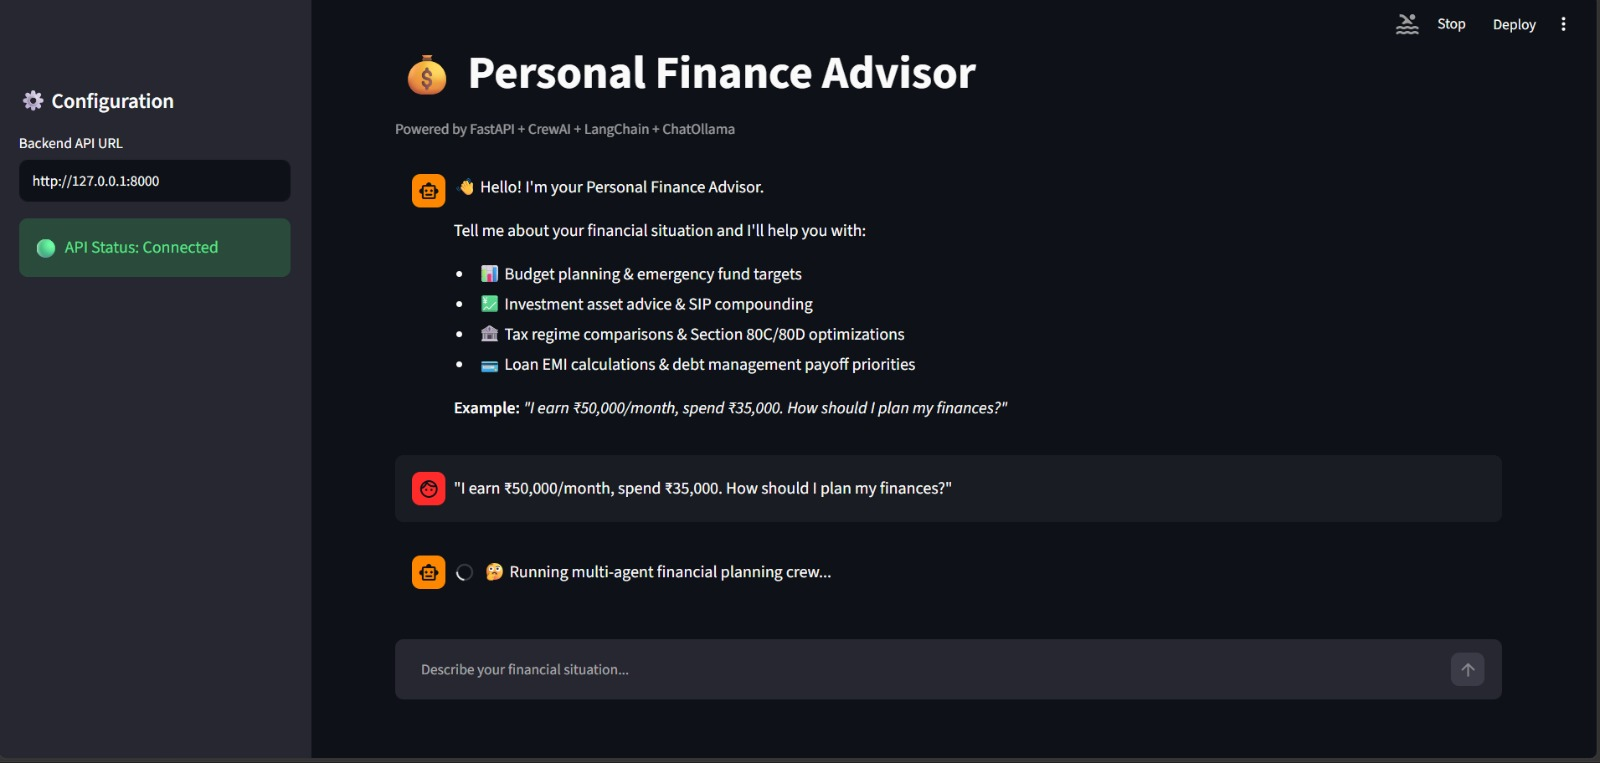
\includegraphics[width=0.95\textwidth]{images/Interface_Financial_Advisor.png}
    \caption{Financial Advisor User Interface}
    \label{fig:streamlit_ui}
\end{figure}

Upon executing the multi-agent n8n workflow, the financial planner agent parses and formats the outputs. Figure \ref{fig:output_screenshot} displays the generated client-ready financial advisory report.

\begin{figure}[H]
    \centering
    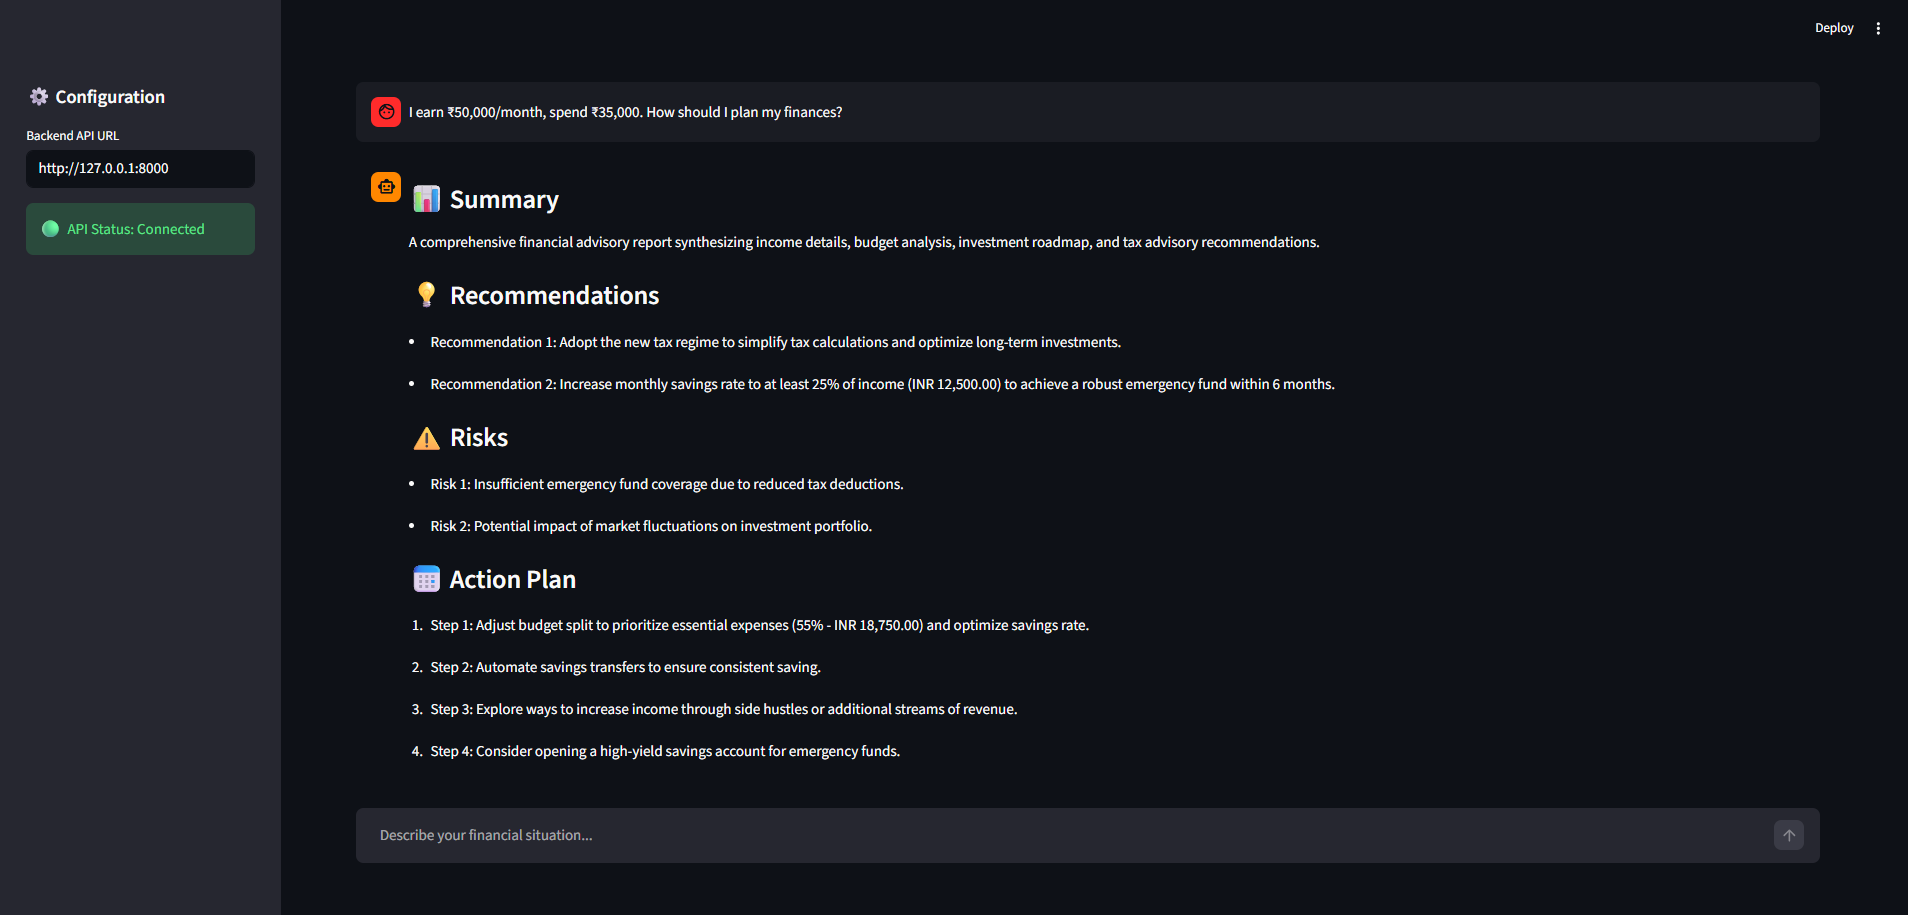
\includegraphics[width=0.95\textwidth]{images/Personal_Finance_Advisor.png} 
    \caption{Generated Financial Advisory Report}
    \label{fig:output_screenshot}
\end{figure}

The advisory output compiles recommendations, identifies financial risks (such as high expenditure rates or lack of retirement assets), and outlines an actionable step-by-step financial plan. The integration of custom calculators ensures that the LLM's natural language advice is grounded in verified, mathematical calculations. Listing \ref{lst:json_output} represents a sample JSON response returned by the system.

\begin{lstlisting}[language=json, caption=JSON Advisory Report Response, label=lst:json_output]
{
  "summary": "Calculated budget with 50-30-20 splits based on monthly income of INR 50,000.00 and expenses of INR 30,000.00. Investment parameters were missing and noted in the report.",
  "recommendations": [
    "Aim to invest your surplus of INR 20,000.00 to build long-term wealth.",
    "Allocate INR 25,000.00 to Needs, INR 15,000.00 to Wants, and INR 10,000.00 to Savings.",
    "Build a 6-month emergency fund target of INR 180,000.00."
  ],
  "risks": [
    "Your current savings rate is 40.00% which is good, but keeping surplus in cash risks inflation erosion.",
    "No investment, tax optimization, or debt data was supplied."
  ],
  "action_plan": [
    "Review your monthly expenses to find areas where you can reduce wants.",
    "Define your SIP goals and provide monthly investment details to run the SIP calculator.",
    "Establish your emergency fund in a liquid savings account."
  ]
}
\end{lstlisting}

This multi-agent sequential pipeline ensures that calculations from the Budget Agent are passed directly into the context of the Investment and Debt Agents, maintaining contextual alignment across all calculations.

\chapter{Future Scope}
While the current implementation establishes a solid, privacy-first personal financial advisory chatbot, several key enhancements remain open for future development:

\begin{enumerate}
    \item \textbf{Real-Time Market Data APIs}: Currently, the Investment Agent uses static compound interest formulas and user-input estimated return rates. In future iterations, connecting this agent to live market data feeds (such as Yahoo Finance, Zerodha, or Alpha Vantage APIs) will allow the system to fetch actual dividend yields, current stock prices, and historical mutual fund returns, generating reports grounded in current market conditions.
    \item \textbf{Automated Bank Feed Integration}: Rather than requiring users to manually input monthly income and expense metrics, the chatbot can be integrated with secure financial messaging and open-banking systems, such as the Account Aggregator (AA) framework in India. This would allow the system to securely ingest monthly transaction logs, automatically parsing and categorizing spending habits using classification models before computing budget margins.
    \item \textbf{Dynamic Charting and Visual Reporting}: The text-based report can be enhanced by integrating dynamic charting libraries (such as Plotly or Chart.js) directly within the Streamlit user interface or n8n dashboard. This would provide interactive representations of 50-30-20 budget allocations (pie charts), SIP wealth accumulation curves (line charts comparing invested capital vs wealth gained), and loan amortization schedules (bar charts detailing principal vs interest splits over time).
    \item \textbf{Retrieval-Augmented Generation (RAG) for Tax Compliance}: The Indian tax structure is subject to changes in annual federal budgets. Integrating a local Vector Database (such as ChromaDB or Qdrant) containing official tax department circulars, policy changes, and investment guidelines would enable the Tax Agent to query relevant compliance documents using semantic search, explaining exactly why a certain deduction path is recommended.
\end{enumerate}

\chapter{Conclusion}
This project successfully demonstrates the design and execution of a local, privacy-first personal financial advisory chatbot using a multi-agent sequential workflow. By combining n8n visual automation, CrewAI agent orchestration, and local Ollama model hosting (\texttt{llama3.2:3b}), the system eliminates recurrent cloud subscription API costs while securing sensitive financial parameters. 

The implementation highlights several key technical achievements:
\begin{enumerate}
    \item \textbf{Addressing Math Hallucinations}: By integrating dedicated JavaScript calculators, the system grounds the natural language capabilities of the LLM in verified mathematical formulas. This eliminates errors where the model tries to compute compound interest or loan amortization directly.
    \item \textbf{Type-Safety in Tool Calling}: Local, lightweight language models often output numerical arguments wrapped in string quotes or omit required inputs. By creating a relaxed validation schema of \texttt{["number", "string", "null"]} and implementing explicit type coercion and fallback regex parsing in the tool scripts, we prevent execution crashes and make the system highly resilient.
    \item \textbf{Privacy by Design}: Financial information is highly sensitive. Running the entire agent workflow locally means that user data is never uploaded to commercial servers or cloud APIs, adhering to strict data sovereignty and privacy guidelines.
    \item \textbf{Cohesive Multi-Agent Orchestration}: Developing a sequential pipeline ensures that calculations from the Budget Agent are directly available to the subsequent Investment, Debt, and Tax Agents, allowing for contextually aligned planning that matches the user's cash flow surplus.
\end{enumerate}

In summary, the chatbot successfully bridges the gap between manual financial spreadsheets and expensive commercial wealth management software, offering a secure, automated, and personalized conversational advisor.

\chapter{References}
\begingroup
\renewcommand{\chapter}[2]{}% Redefine chapter command to prevent double-headings
\nocite{*}
\bibliographystyle{plain}
\bibliography{references}
\endgroup


\end{document}
